\section{Features}

A more extensive list of search features can be shown using the \texttt{--help}
switch.

\subsection{Search Algorithms}
\label{sub:Search Algorithms}

The solver implements the following search methods:

\begin{itemize}
  \item Uninformed
  \begin{itemize}
    \item Breadth-First Search, \texttt{BFS}
    \item Depth-First Search, \texttt{DFS}
    \item Depth-Limited Search, \texttt{DLS,CUS1}
    \item Bogosort Search, \texttt{BOGO,CUS3}
  \end{itemize}
  \item Informed:
  \begin{itemize}
    \item Greedy Best-First Search, \texttt{GBFS}
    \item A-Star Search, \texttt{AS}
    \item Iterative-Deepening A-Star Search, \texttt{IDAS,CUS2}
  \end{itemize}
\end{itemize}

Note that \texttt{DLS} and \texttt{IDAS} searches can utilise the
\texttt{--threshold} switch when executing, which will specify the
maximum node path cost to traverse (for \texttt{DLS}) or the limit
to the evaluation function result that will be accepted for searches
(for \texttt{IDAS}), that is:

\begin{center}
  \vspace{1em}
  \noindent
  $pc(n) < threshold_{DLS}$
  \\
  $f(n) < threshold_{IDAS}$
  \vspace{1em}
\end{center}

By default, the heuristic used for informed searches is the Manhattan Distance
heuristic. This can be changed to other heuristics by using the \texttt{--heuristic}
switch and providing one of: \texttt{manhattan}, \texttt{euclidean},
\texttt{manhattan}, or \texttt{misplaced}. Refer to the help for more instructions.


\subsection{Graphical Solver}
\label{sub:Graphical Solver}


A graphical solver can show both the search method solving the puzzle
as well as a solution to the puzzle where state's in the node tree are
represented by the $n$ by $m$ matrix as coloured tiles. See Figure~\ref{fig:gui}.

\begin{figure}[h!]
  \centering
  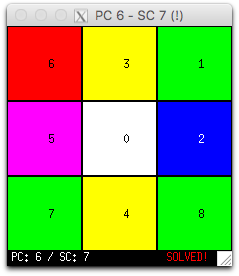
\includegraphics{gui.png}
  \caption{GUI of a puzzle solver}
  \label{fig:gui}
\end{figure}

You can initate the GUI by using the following switches:

\begin{itemize}
  \item \texttt{\bfseries --gui=solved}
  Show only the solved puzzle. Traverse the search tree from the root node to
  the goal node using the \texttt{B} or $\uparrow$ Keys and down the tree using
  the \texttt{F} or $\downarrow$ Keys
  \item \texttt{\bfseries --gui=solving}\footnote{Not that when using the
  solving GUI, the search algorithm may appear to be slower than when not using
  the GUI. This is due to render lag caused by X11, used to render the GUI.}
  Show the search algorithm solving the puzzle. When solving the GUI will not be
  responsive, so should you want to quit the solver, you will need to terminate
  at the command line using \texttt{\^{}C}
\end{itemize}
